
\begin{minipage}{0.48\linewidth}


Au rugby, une pénalité est un tir entre deux perches distantes de 4m. Avec les moyens techniques numériques de la télévision, lors des matchs de rugby, on peut lire les indications suivantes :


Quelle  est l'amplitude de l'angle de frappe pour que le joueur marque la pénalité ?


\includegraphics[scale=0.8]{qrcodePenalite.png} 

\end{minipage}
\hfill
\begin{minipage}{0.48\linewidth}
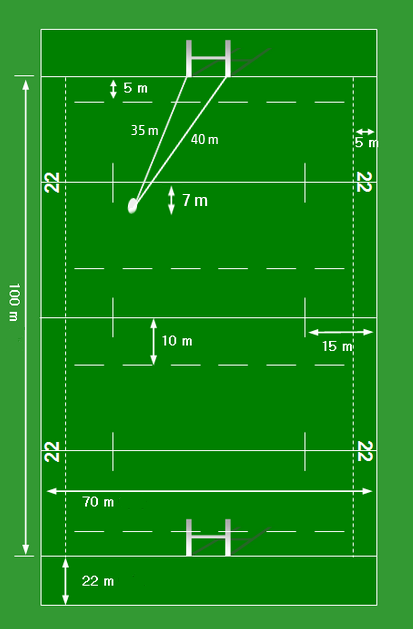
\includegraphics[scale=0.8]{TR-219.png} 
\end{minipage}